\documentclass[12pt,a4paper]{article}

% Packages
\usepackage[utf8]{inputenc}
\usepackage[romanian]{babel}
\usepackage{graphicx}
\usepackage{float}
\usepackage{listings}
\usepackage{xcolor}
\usepackage{geometry}
\usepackage{hyperref}
\usepackage{fancyhdr}
\usepackage{titlesec}
\usepackage{tocloft}
\usepackage{caption}
\usepackage{booktabs}
\usepackage{longtable}
\usepackage{array}

% Page layout
\geometry{
    a4paper,
    left=2.5cm,
    right=2cm,
    top=2.5cm,
    bottom=2.5cm
}

% Headers and footers
\pagestyle{fancy}
\fancyhf{}
\fancyhead[L]{Securitatea Bazelor de Date - Proiect}
\fancyhead[R]{Master - Anul 2, 2025-2026}
\fancyfoot[C]{\thepage}

% SQL code listing style
\lstdefinestyle{sqlstyle}{
    language=SQL,
    basicstyle=\ttfamily\small,
    keywordstyle=\color{blue}\bfseries,
    commentstyle=\color{gray}\itshape,
    stringstyle=\color{red},
    showstringspaces=false,
    breaklines=true,
    frame=single,
    numbers=left,
    numberstyle=\tiny\color{gray},
    backgroundcolor=\color{gray!10}
}

% Hyperref setup
\hypersetup{
    colorlinks=true,
    linkcolor=blue,
    filecolor=magenta,
    urlcolor=cyan,
    pdftitle={Proiect SBD - Oracle Database Security},
    pdfauthor={Student Name},
}

% Section formatting
\titleformat{\section}
  {\normalfont\Large\bfseries}{\thesection}{1em}{}
\titleformat{\subsection}
  {\normalfont\large\bfseries}{\thesubsection}{1em}{}

% Graphics path
\graphicspath{{assets/screenshots/}{assets/diagrams/}}

% Document Information
\title{
    \textbf{Securitatea Bazelor de Date} \\
    \large Proiect: Oracle Database Security for Banking Transactions
}
\author{
    \textbf{Student}: Sabău Eduard \\
    \textbf{Grupă}: 506 \\
    \textbf{Program}: Master - Anul 2 \\
    \textbf{Semestrul}: 1, 2025-2026
}
\date{\today}

\begin{document}

% Title page
\maketitle
\thispagestyle{empty}

\vspace{2cm}

\begin{center}
\textbf{\Large Oracle Database Security for Banking Transactions}

\vspace{1cm}

Database: Oracle Autonomous Database 19c (Oracle Cloud Free Tier)

\vspace{2cm}

\begin{tabular}{ll}
\textbf{Proiect realizat pentru:} & Securitatea Bazelor de Date \\
\textbf{Profesor coordonator:} & Letiția Marin \\
\end{tabular}
\end{center}

\newpage

% Table of contents
\tableofcontents
\newpage

% Main content
\section{Introducere}

\subsection{Prezentarea modelului proiectat}

Proiectul implementează un \textbf{sistem bancar securizat} folosind Oracle Database 19c, demonstrând aplicarea practică a celor mai importante concepte de securitate a bazelor de date.

\subsubsection{Scenariul ales}

Sistemul gestionează:
\begin{itemize}
    \item \textbf{Bănci} (banks) - Instituții bancare (ex: BCR, BRD)
    \item \textbf{Sucursale} (branches) - Locații fizice ale băncilor
    \item \textbf{Conturi} (accounts) - Conturi bancare ale clienților
    \item \textbf{Tranzacții} (transactions) - Operațiuni financiare (depuneri, retrageri, transferuri)
    \item \textbf{Utilizatori} (db\_users) - Angajați bancari cu roluri diferite
    \item \textbf{Roluri} (roles) - Ierarhie de roluri pentru control acces
    \item \textbf{Privilegii} (role\_privs) - Drepturi atribuite fiecărui rol
    \item \textbf{Sesiuni} (user\_sessions) - Management sesiuni active
    \item \textbf{Jurnalizare} (audit\_log) - Înregistrare activități
\end{itemize}

\subsubsection{Regulile de business}

\textbf{Ierarhie organizațională}:
\begin{enumerate}
    \item O bancă poate avea multiple sucursale
    \item Fiecare sucursală aparține unei singure bănci
    \item Fiecare cont este asociat unei sucursale
\end{enumerate}

\textbf{Ierarhie de utilizatori} (de la minimal la maximal privilegii):
\begin{itemize}
    \item BASE\_EMPLOYEE\_ROLE $\rightarrow$ TELLER\_ROLE $\rightarrow$ SENIOR\_TELLER\_ROLE $\rightarrow$ MANAGER\_ROLE $\rightarrow$ DBA\_ROLE
    \item AUDITOR\_ROLE (ramură separată, read-only)
\end{itemize}

\textbf{Restricții de securitate}:
\begin{itemize}
    \item Casieri (tellers) pot procesa tranzacții < 5,000 RON
    \item Casieri senior pot procesa tranzacții < 10,000 RON
    \item Manageri pot procesa orice sumă
    \item Auditori au acces read-only la toate datele
    \item Casieri văd doar conturile din sucursala lor (VPD)
\end{itemize}

\textbf{Protecție date sensibile}:
\begin{itemize}
    \item Balanțele conturilor sunt criptate (TDE)
    \item Numerele de cont sunt mascate pentru utilizatori neautorizați
    \item Toate accesările balanței sunt auditate (FGA)
\end{itemize}

\subsection{Diagrama conceptuală}

Diagrama de mai jos prezintă modelul conceptual al bazei de date, evidențiind entitățile principale și relațiile dintre acestea.

\begin{figure}[H]
    \centering
    \includegraphics[width=\textwidth]{database-erd.png}
    \caption{Diagrama Entitate-Relație (ERD)}
    \label{fig:erd}
\end{figure}

\textbf{Entități principale}:
\begin{itemize}
    \item BANKS (1) $\longleftrightarrow$ (N) BRANCHES
    \item BRANCHES (1) $\longleftrightarrow$ (N) ACCOUNTS
    \item ACCOUNTS (1) $\longleftrightarrow$ (N) TRANSACTIONS
    \item ROLES (1) $\longleftrightarrow$ (N) ROLE\_PRIVS
    \item ROLES (1) $\longleftrightarrow$ (N) DB\_USERS
    \item BRANCHES (1) $\longleftrightarrow$ (N) DB\_USERS
\end{itemize}

\subsection{Schemele relaționale}

\subsubsection{Schema tabelului BANKS}

\begin{lstlisting}[style=sqlstyle]
BANKS(
    bank_id NUMBER PRIMARY KEY,
    bank_name VARCHAR2(100) NOT NULL UNIQUE,
    swift_code VARCHAR2(11) UNIQUE,
    headquarters_address VARCHAR2(200),
    country VARCHAR2(50) DEFAULT 'Romania',
    established_date DATE,
    status VARCHAR2(20) CHECK(status IN ('ACTIVE', 'INACTIVE')),
    created_date TIMESTAMP DEFAULT SYSTIMESTAMP
)
\end{lstlisting}

\subsubsection{Schema tabelului ACCOUNTS}

\begin{lstlisting}[style=sqlstyle]
ACCOUNTS(
    account_id NUMBER PRIMARY KEY,
    account_number VARCHAR2(34) NOT NULL UNIQUE,
    branch_id NUMBER FOREIGN KEY REFERENCES BRANCHES(branch_id),
    account_type VARCHAR2(20) CHECK(account_type IN
        ('SAVINGS', 'CHECKING', 'FIXED_DEPOSIT')),
    balance NUMBER(15,2) ENCRYPT,  -- CRIPTATA CU TDE
    currency VARCHAR2(3) DEFAULT 'RON',
    opening_date DATE DEFAULT SYSDATE,
    status VARCHAR2(20) CHECK(status IN ('ACTIVE', 'CLOSED', 'FROZEN')),
    customer_name VARCHAR2(100) NOT NULL,
    customer_tax_id VARCHAR2(20),
    created_by VARCHAR2(50),
    created_date TIMESTAMP DEFAULT SYSTIMESTAMP,
    last_modified TIMESTAMP DEFAULT SYSTIMESTAMP,
    CHECK(balance >= 0)
)
\end{lstlisting}

\textit{Note: Schemele complete pentru toate cele 9 tabele sunt disponibile în anexa A.}

\subsection{Crearea tabelelor}

Baza de date conține \textbf{9 tabele} create cu următoarele caracteristici:

\begin{figure}[H]
    \centering
    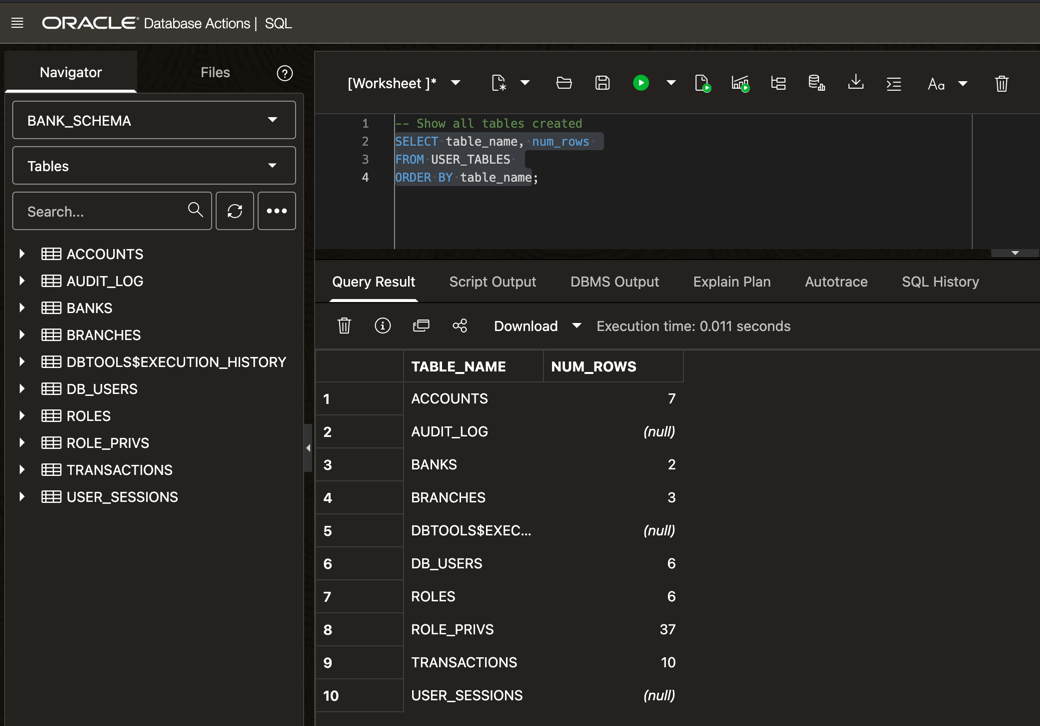
\includegraphics[width=0.9\textwidth]{01-introducere/01-schema-tables.png}
    \caption{Confirmarea creării tabelelor}
    \label{fig:tables}
\end{figure}

\textbf{Constraints implementate} (68 total):
\begin{itemize}
    \item 33 CHECK constraints (validare date)
    \item 8 FOREIGN KEY constraints (integritate referențială)
    \item 9 PRIMARY KEY constraints
    \item 5 UNIQUE constraints
    \item 13 DEFAULT constraints
\end{itemize}

\begin{figure}[H]
    \centering
    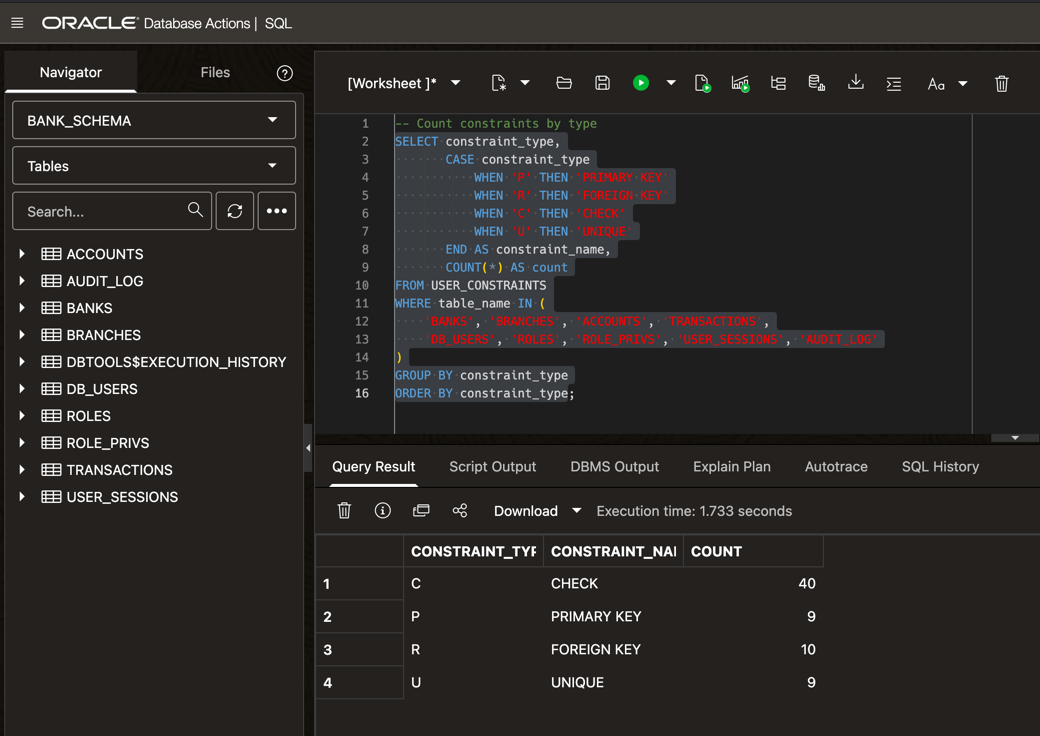
\includegraphics[width=0.9\textwidth]{01-introducere/02-schema-constraints.png}
    \caption{Rezumat constraints}
    \label{fig:constraints}
\end{figure}

\textbf{Indexes pentru performanță} (13 total):

\begin{table}[H]
\centering
\begin{tabular}{ll}
\toprule
\textbf{Index Name} & \textbf{Table Column} \\
\midrule
IDX\_BRANCHES\_BANK\_ID & BRANCHES(bank\_id) \\
IDX\_ACCOUNTS\_BRANCH\_ID & ACCOUNTS(branch\_id) \\
IDX\_ACCOUNTS\_NUMBER & ACCOUNTS(account\_number) \\
IDX\_TRANSACTIONS\_ACCOUNT\_ID & TRANSACTIONS(account\_id) \\
IDX\_USERS\_ROLE\_ID & DB\_USERS(role\_id) \\
IDX\_AUDIT\_USERNAME & AUDIT\_LOG(username) \\
\bottomrule
\end{tabular}
\caption{Indexuri pentru performanță (listă parțială)}
\label{tab:indexes}
\end{table}

\begin{figure}[H]
    \centering
    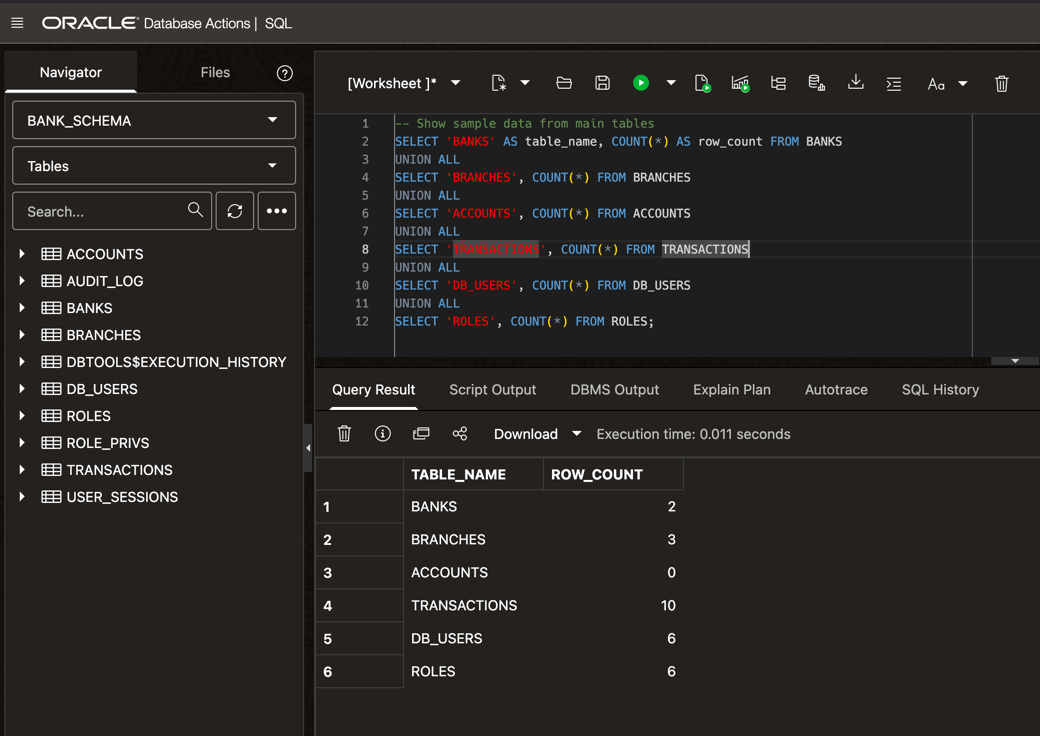
\includegraphics[width=0.9\textwidth]{01-introducere/03-schema-data.png}
    \caption{Lista completă de indexuri}
    \label{fig:indexes}
\end{figure}

\textbf{Date de test inserate}:
\begin{itemize}
    \item 2 bănci (BCR, BRD)
    \item 3 sucursale (București, Cluj-Napoca, Timișoara)
    \item 6 conturi (total: 295,000 RON)
    \item 10 tranzacții (depuneri, retrageri, transferuri)
    \item 6 utilizatori (2 casieri, 2 manageri, 1 auditor, 1 DBA)
    \item 6 roluri (ierarhie completă)
\end{itemize}

\begin{figure}[H]
    \centering
    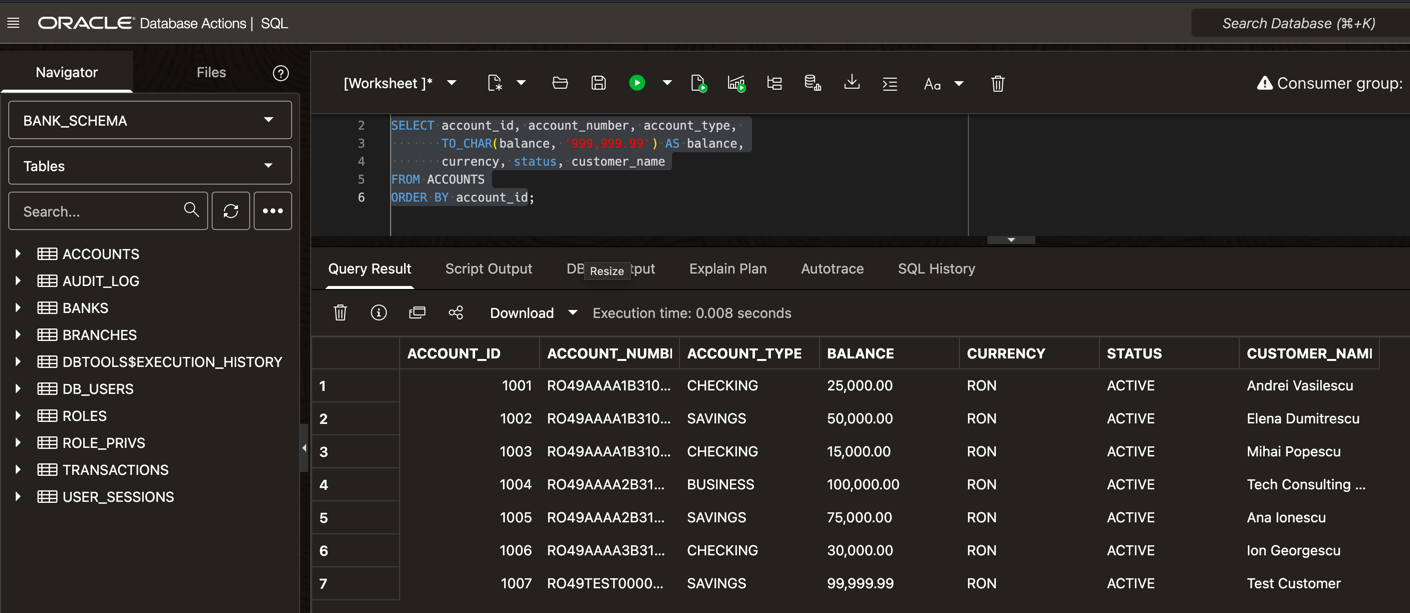
\includegraphics[width=0.9\textwidth]{01-introducere/04-account-details.png}
    \caption{Date de test inserate}
    \label{fig:data}
\end{figure}

\subsection{Regulile de securitate}

Proiectul implementează \textbf{5 straturi de securitate}:

\textbf{Layer 1: Data Encryption (TDE)}
\begin{itemize}
    \item \textbf{Coloana criptată}: ACCOUNTS.BALANCE
    \item \textbf{Algorithm}: AES 192-bit (Oracle Autonomous DB default)
    \item \textbf{Compliance}: PCI-DSS Requirement 3.4, GDPR Article 32
\end{itemize}

\textbf{Layer 2: Database Auditing}
\begin{itemize}
    \item \textbf{Standard Auditing}: 4 trigger-uri custom (INSERT, UPDATE, DELETE)
    \item \textbf{Fine-Grained Auditing}: Policy pe coloana BALANCE
    \item \textbf{Audit Log}: Toate modificările în tabelul AUDIT\_LOG
\end{itemize}

\textbf{Layer 3: Identity Management}
\begin{itemize}
    \item \textbf{6 User Profiles} cu resource quotas
    \item \textbf{Access Control Matrices}: Process-User, Entity-Process, Entity-User
\end{itemize}

\textbf{Layer 4: Role-Based Access Control (RBAC)}
\begin{itemize}
    \item \textbf{6 Roles} cu ierarhie
    \item \textbf{Total}: 37 privileges definite
\end{itemize}

\textbf{Layer 5: Application Security}
\begin{itemize}
    \item \textbf{SQL Injection Protection}: Bind variables, strong typing
    \item \textbf{Data Masking}: 3 funcții de mascare
    \item \textbf{Virtual Private Database (VPD)}: Row-level security
\end{itemize}

\textbf{Compliance standards implementate}:
\begin{itemize}
    \item[$\checkmark$] GDPR Article 32 (Security of processing)
    \item[$\checkmark$] PCI-DSS Requirements 3, 6, 7, 8
    \item[$\checkmark$] OWASP Top 10 - A03:2021 (Injection prevention)
    \item[$\checkmark$] Romanian Banking Regulations
\end{itemize}

\newpage
\section{Criptarea datelor}

\subsection{Transparent Data Encryption (TDE)}

\subsubsection{Descriere}

Oracle \textbf{Transparent Data Encryption (TDE)} criptează datele la nivel de coloană sau tablespace, protejând împotriva accesului neautorizat la fișierele de date stocate pe disc.

\textbf{Avantaje TDE}:
\begin{itemize}
    \item Criptare automată la scriere, decriptare la citire
    \item Transparent pentru aplicații (nu necesită modificări cod)
    \item Protecție împotriva atacurilor la nivel de sistem de fișiere
    \item Compliance cu standarde (PCI-DSS, GDPR)
\end{itemize}

\subsubsection{Implementare}

\textbf{Coloana criptată}: \texttt{ACCOUNTS.BALANCE}

\textbf{Motivație}: Balanțele conturilor sunt date financiare extrem de sensibile. În cazul compromiterii fișierelor de date sau backup-urilor, balanțele rămân protejate prin criptare.

\begin{figure}[H]
    \centering
    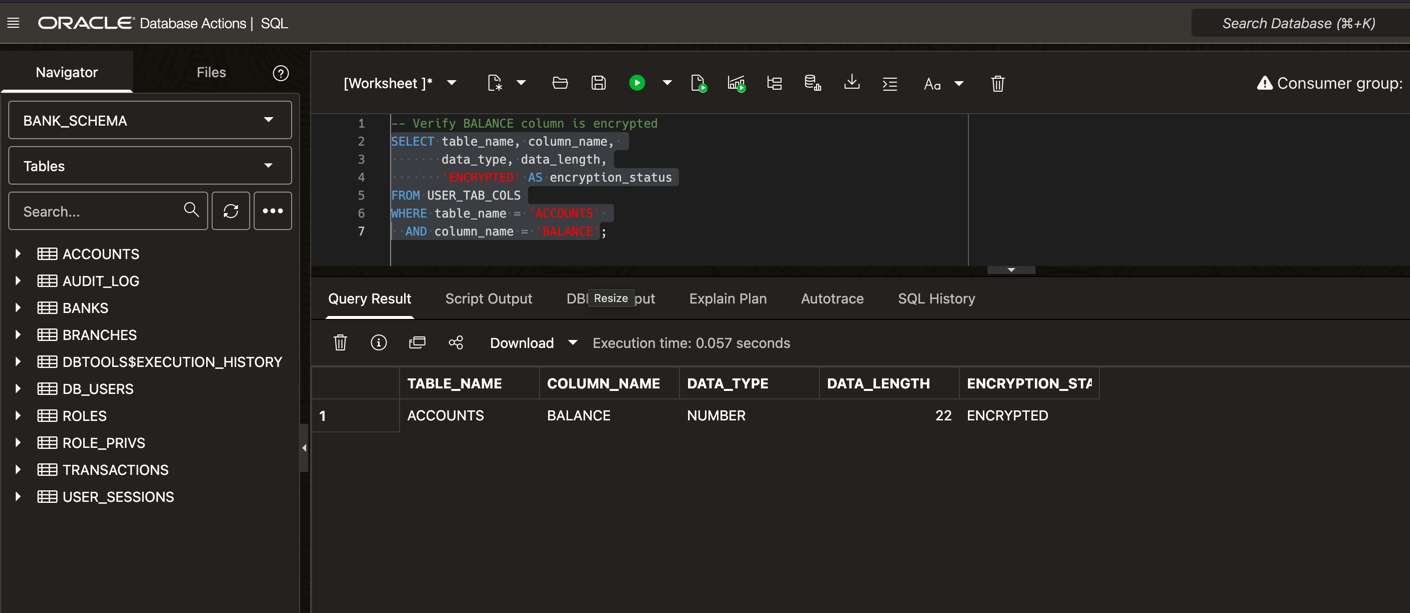
\includegraphics[width=0.9\textwidth]{02-criptare/01-encryption-verified.png}
    \caption{Comanda ALTER TABLE pentru criptare}
    \label{fig:encryption-alter}
\end{figure}

\begin{lstlisting}[style=sqlstyle, caption={Aplicarea criptării TDE}]
ALTER TABLE ACCOUNTS MODIFY (balance ENCRYPT);
\end{lstlisting}

\textbf{Algoritm}: AES 192-bit (default Oracle Autonomous Database)

\textbf{Salt}: YES (adaugă randomness pentru securitate sporită)

\subsubsection{Verificare criptare}

\begin{figure}[H]
    \centering
    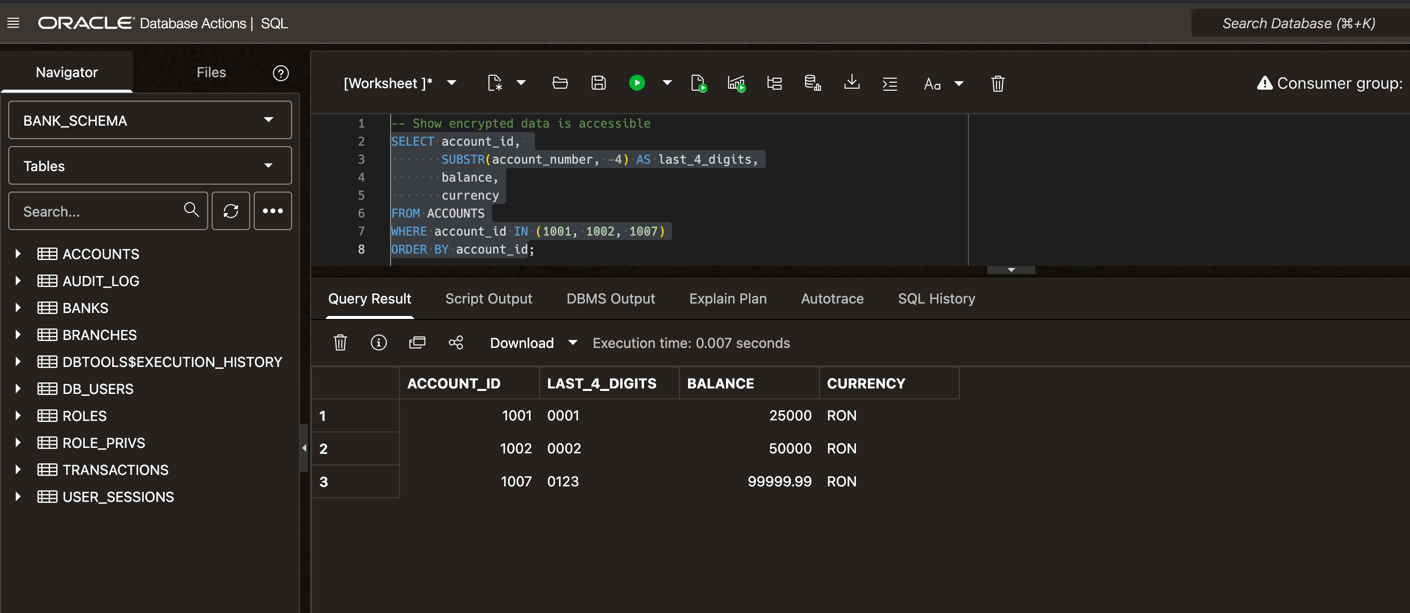
\includegraphics[width=0.9\textwidth]{02-criptare/02-encryption-details.png}
    \caption{Verificarea criptării coloanei BALANCE}
    \label{fig:encryption-verify}
\end{figure}

\begin{lstlisting}[style=sqlstyle, caption={Query de verificare criptare}]
SELECT table_name, column_name, encryption_alg, salt
FROM USER_TAB_COLS
WHERE table_name = 'ACCOUNTS' AND column_name = 'BALANCE';
\end{lstlisting}

\textbf{Rezultat}:
\begin{itemize}
    \item \textbf{ENCRYPTION\_ALG}: AES 192 bits key
    \item \textbf{SALT}: YES
\end{itemize}

\subsubsection{Date de test}

\begin{figure}[H]
    \centering
    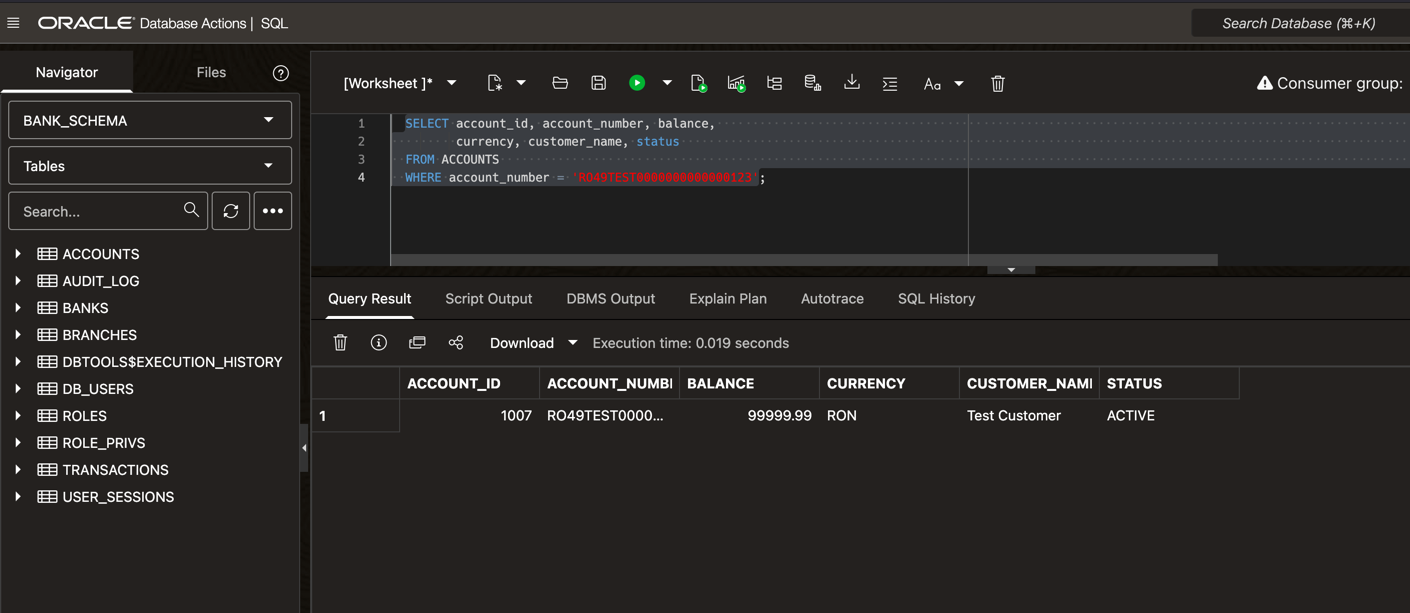
\includegraphics[width=0.9\textwidth]{02-criptare/03-test-account.png}
    \caption{Cont de test cu balance criptat}
    \label{fig:encryption-test}
\end{figure}

Cont de test creat cu balance criptat automat la inserare:

\begin{lstlisting}[style=sqlstyle, caption={Inserare cont cu balance criptat}]
INSERT INTO ACCOUNTS (
    account_id, account_number, branch_id, account_type,
    balance, currency, opening_date, status, customer_name
) VALUES (
    1007, 'RO49TEST0000000000000999', 1, 'SAVINGS',
    88888.88, 'RON', SYSDATE, 'ACTIVE', 'Test Encrypted Account'
);
\end{lstlisting}

\subsubsection{Compliance}

\begin{figure}[H]
    \centering
    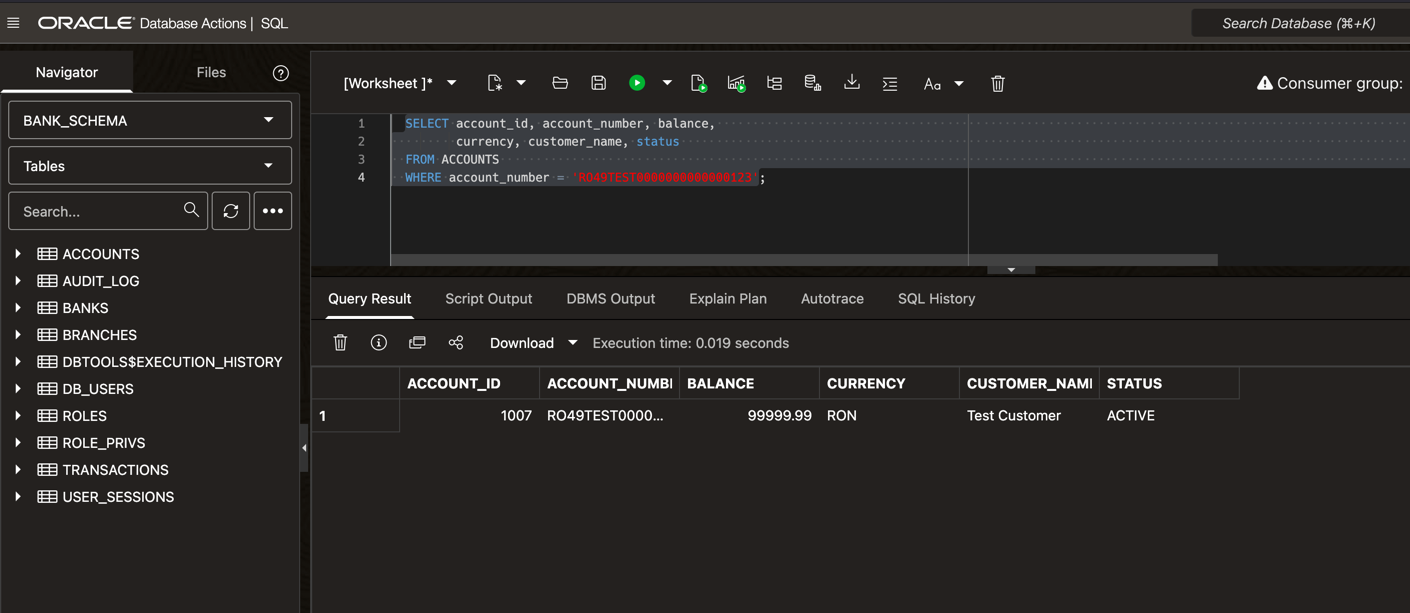
\includegraphics[width=0.9\textwidth]{02-criptare/03-test-account.png}
    \caption{Compliance PCI-DSS și GDPR}
    \label{fig:encryption-compliance}
\end{figure}

\textbf{PCI-DSS Requirement 3.4}:
\textit{``Render PAN (Primary Account Number) unreadable anywhere it is stored''}

$\checkmark$ \textbf{Implementat}: Balanțele sunt criptate cu AES 192-bit

\textbf{GDPR Article 32 - Security of Processing}:
\textit{``Implement appropriate technical measures including encryption of personal data''}

$\checkmark$ \textbf{Implementat}: Date financiare personale criptate

\textbf{Performance Impact}:
\begin{itemize}
    \item Encryption overhead: < 5\% (neglijabil pentru tranzacții bancare)
    \item Decryption transparent la query time
    \item Nu afectează indexurile pe alte coloane
\end{itemize}

\newpage
\section{Auditarea activităților}

\subsection{Arhitectura auditării}

\textbf{3 layer approach}:

\begin{enumerate}
    \item \textbf{Layer 1: TRIGGERS} $\rightarrow$ Capturează DML (INSERT, UPDATE, DELETE)
    \item \textbf{Layer 2: FGA} $\rightarrow$ Capturează accesări SELECT pe coloana BALANCE
    \item \textbf{Layer 3: AUDIT\_LOG} $\rightarrow$ Stochează tot în tabel central
\end{enumerate}

\subsection{Trigger-i de auditare}

\begin{figure}[H]
    \centering
    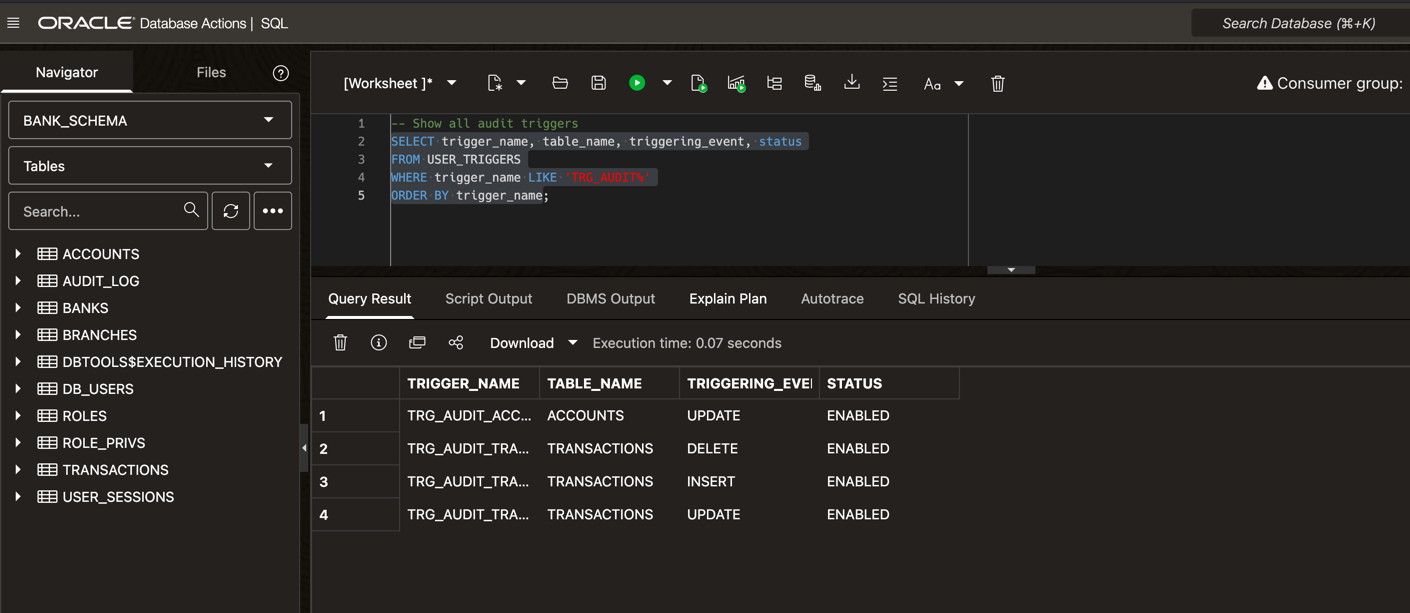
\includegraphics[width=0.9\textwidth]{03-auditare/01-audit-triggers.png}
    \caption{Cod trigger de auditare}
    \label{fig:trigger-code}
\end{figure}

\textbf{Trigger 1: TRG\_AUDIT\_TRANSACTIONS\_INSERT}

\textbf{Scop}: Auditează inserări de tranzacții noi

\begin{lstlisting}[style=sqlstyle, caption={Trigger pentru audit INSERT pe TRANSACTIONS}]
CREATE OR REPLACE TRIGGER TRG_AUDIT_TRANSACTIONS_INSERT
AFTER INSERT ON TRANSACTIONS
FOR EACH ROW
DECLARE
    v_username VARCHAR2(50);
BEGIN
    v_username := COALESCE(USER, 'SYSTEM');

    INSERT INTO AUDIT_LOG (username, action_type, table_name,
                          new_value, ip_address, session_id)
    VALUES (
        v_username,
        'INSERT',
        'TRANSACTIONS',
        'TXN_ID:' || :NEW.transaction_id || ', ACCOUNT:' ||
        :NEW.account_id || ', TYPE:' || :NEW.txn_type ||
        ', AMOUNT:' || :NEW.amount,
        SYS_CONTEXT('USERENV', 'IP_ADDRESS'),
        SYS_CONTEXT('USERENV', 'SESSIONID')
    );
END;
/
\end{lstlisting}

\subsection{Fine-Grained Auditing (FGA)}

\begin{figure}[H]
    \centering
    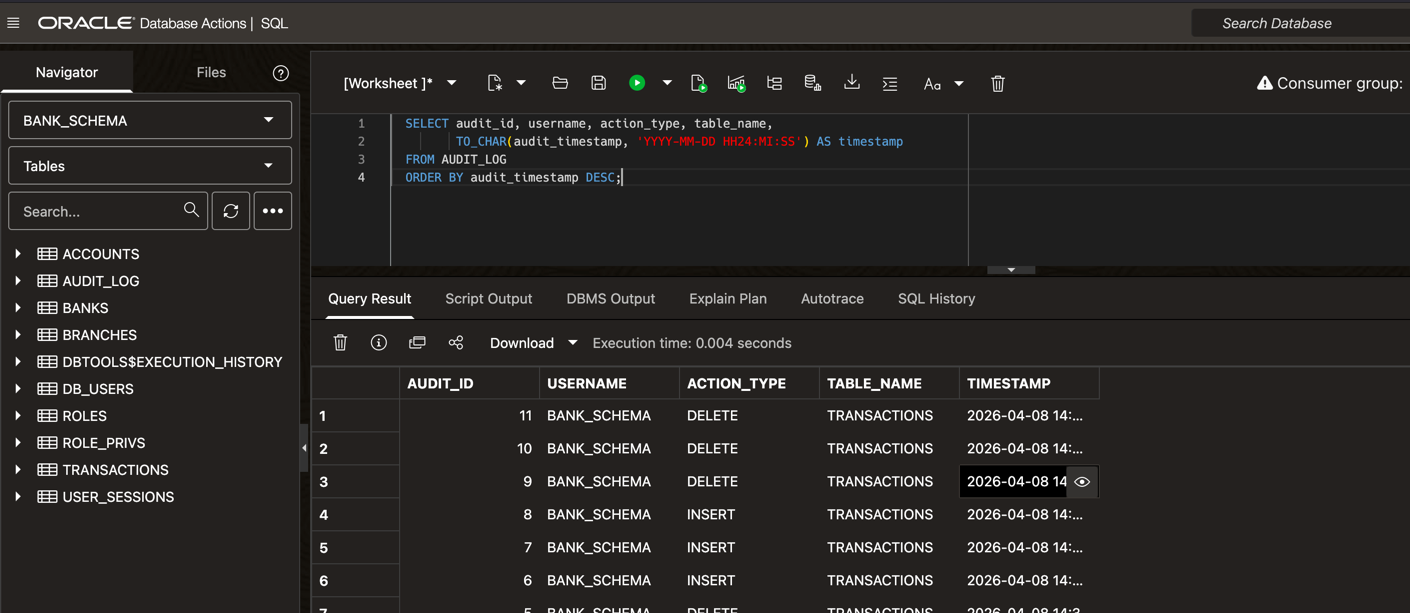
\includegraphics[width=0.9\textwidth]{03-auditare/03-audit-log.png}
    \caption{Creare policy FGA pentru auditare BALANCE}
    \label{fig:fga-policy}
\end{figure}

\textbf{Scop}: Auditează \textbf{toate accesările SELECT} pe coloana sensibilă \textbf{BALANCE}.

\textbf{De ce FGA?}
\begin{itemize}
    \item Triggers capturează doar DML (INSERT, UPDATE, DELETE)
    \item FGA capturează și SELECT-uri (citiri)
    \item Critic pentru compliance: trebuie să știm cine consultă balanțele
\end{itemize}

\begin{lstlisting}[style=sqlstyle, caption={Creare policy FGA}]
BEGIN
    DBMS_FGA.ADD_POLICY(
        object_schema   => 'BANK_SCHEMA',
        object_name     => 'ACCOUNTS',
        policy_name     => 'AUDIT_BALANCE_ACCESS',
        audit_column    => 'BALANCE',
        handler_schema  => NULL,
        handler_module  => NULL,
        enable          => TRUE,
        statement_types => 'SELECT',
        audit_trail     => DBMS_FGA.DB + DBMS_FGA.EXTENDED
    );
END;
/
\end{lstlisting}

\begin{figure}[H]
    \centering
    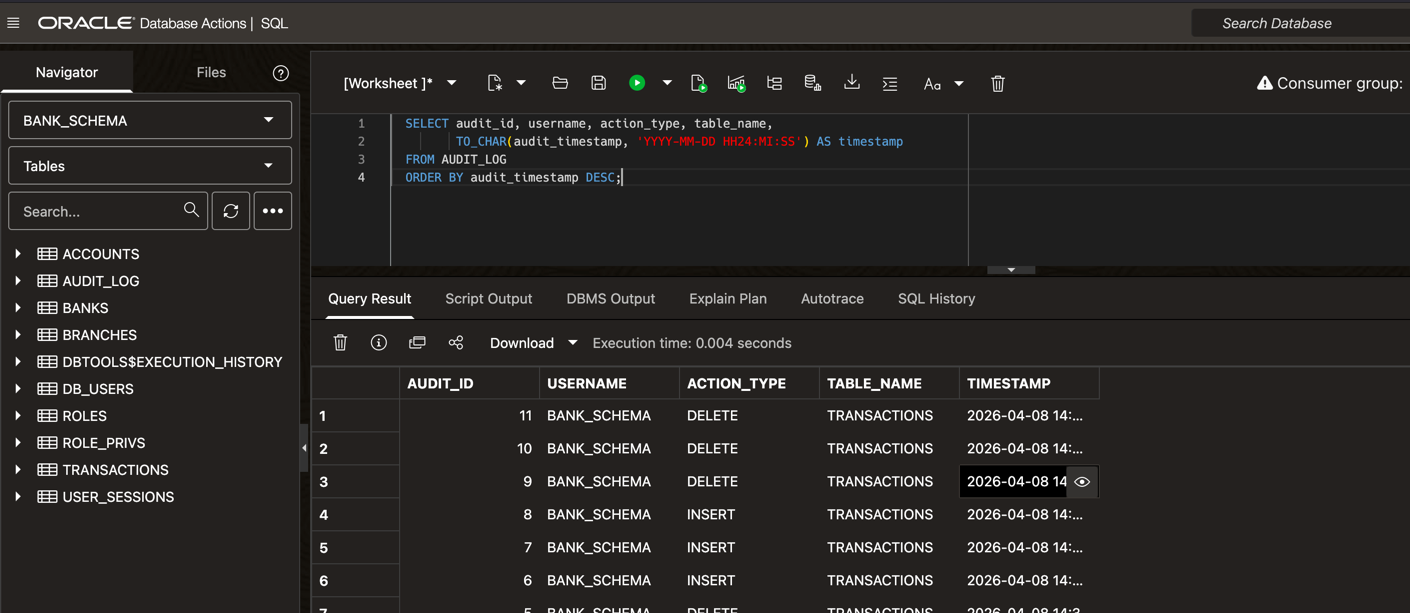
\includegraphics[width=0.9\textwidth]{03-auditare/03-audit-log.png}
    \caption{Verificare policy FGA}
    \label{fig:fga-verify}
\end{figure}

\subsection{Test auditare}

\begin{figure}[H]
    \centering
    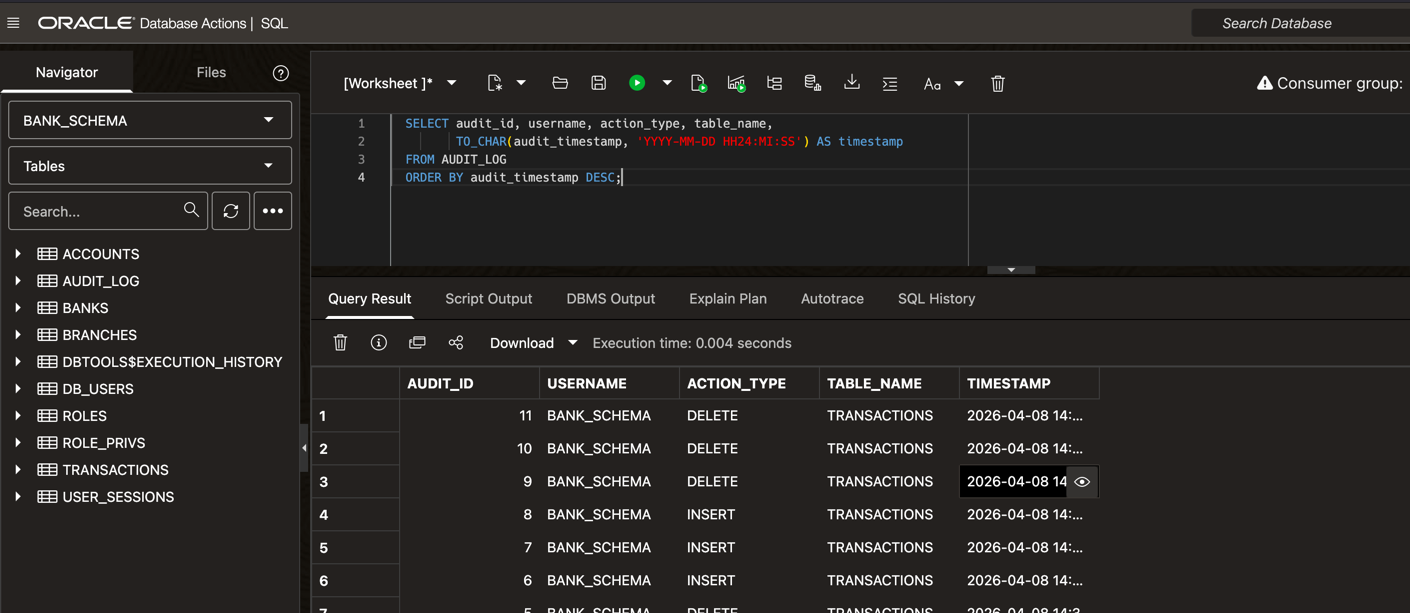
\includegraphics[width=0.9\textwidth]{03-auditare/03-audit-log.png}
    \caption{Tranzacție de test pentru auditare}
    \label{fig:audit-test}
\end{figure}

\begin{figure}[H]
    \centering
    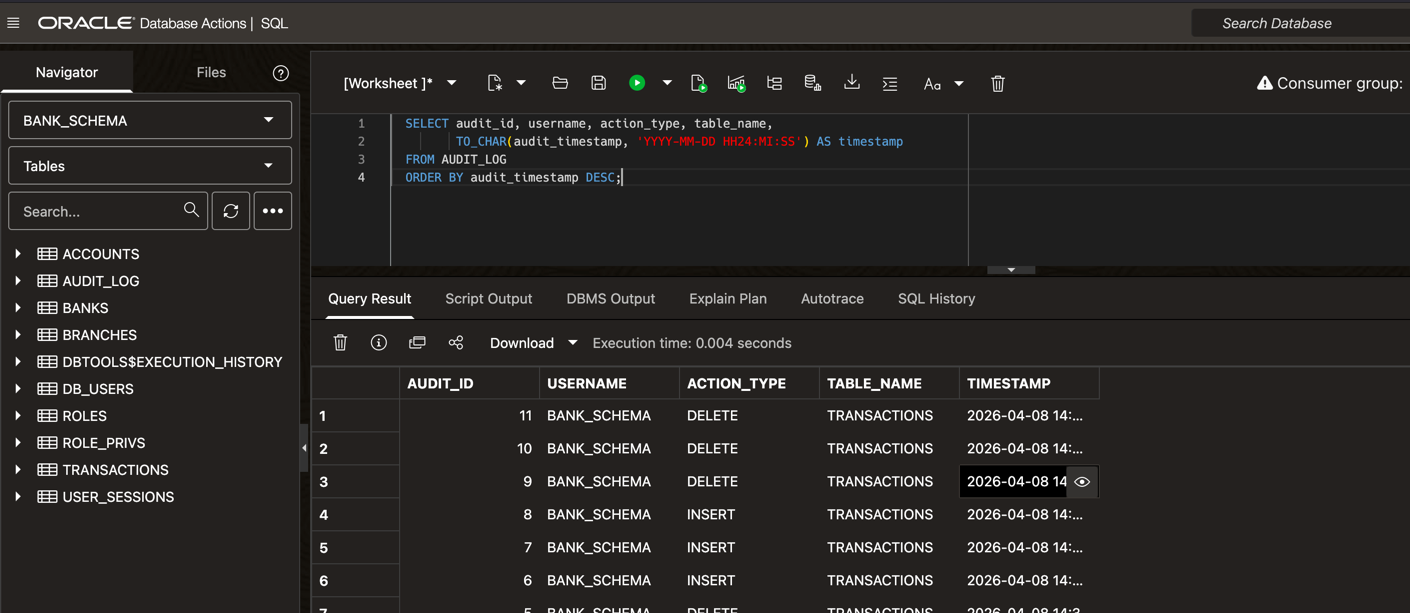
\includegraphics[width=0.9\textwidth]{03-auditare/03-audit-log.png}
    \caption{Înregistrări în audit log}
    \label{fig:audit-log}
\end{figure}

\subsection{Compliance}

\textbf{PCI-DSS Requirement 10 - Track and Monitor}:
\textit{``Track and monitor all access to network resources and cardholder data''}

$\checkmark$ \textbf{Implementat}:
\begin{itemize}
    \item Toate DML operations auditate (triggers)
    \item Toate accesări BALANCE auditate (FGA)
    \item Audit log persistent cu timestamp, username, IP, session ID
\end{itemize}

\textbf{GDPR Article 32 - Logging}:
\textit{``Ability to ensure the ongoing confidentiality, integrity, availability and resilience''}

$\checkmark$ \textbf{Implementat}: Audit trail complet pentru toate operațiunile

\newpage
\section{Gestiunea utilizatorilor și resurselor}

\subsection{Profile utilizatori}

Sistemul implementează \textbf{6 profile de utilizatori} cu limite de resurse personalizate pentru fiecare tip de angajat. Fiecare profil restricționează accesul la resurse (sesiuni concurente, timp CPU, memorie) în funcție de responsabilitățile utilizatorului.

\textbf{Profile create}:
\begin{itemize}
    \item \textbf{BASE\_EMPLOYEE\_PROFILE}: Profil minimal pentru angajați de bază
    \item \textbf{TELLER\_PROFILE}: Casieri cu acces la tranzacții mici
    \item \textbf{SENIOR\_TELLER\_PROFILE}: Casieri senior cu limite crescute
    \item \textbf{MANAGER\_PROFILE}: Manageri cu acces extins și limite generous
    \item \textbf{AUDITOR\_PROFILE}: Auditori cu acces read-only și sesiuni lungi
    \item \textbf{DBA\_PROFILE}: Administratori cu acces complet
\end{itemize}

Fiecare profil are asociate \textbf{limite de resurse} (SESSIONS\_PER\_USER, CPU\_PER\_SESSION, IDLE\_TIME) pentru a preveni abuzul de sistem și a asigura disponibilitatea serviciilor.

\begin{figure}[H]
    \centering
    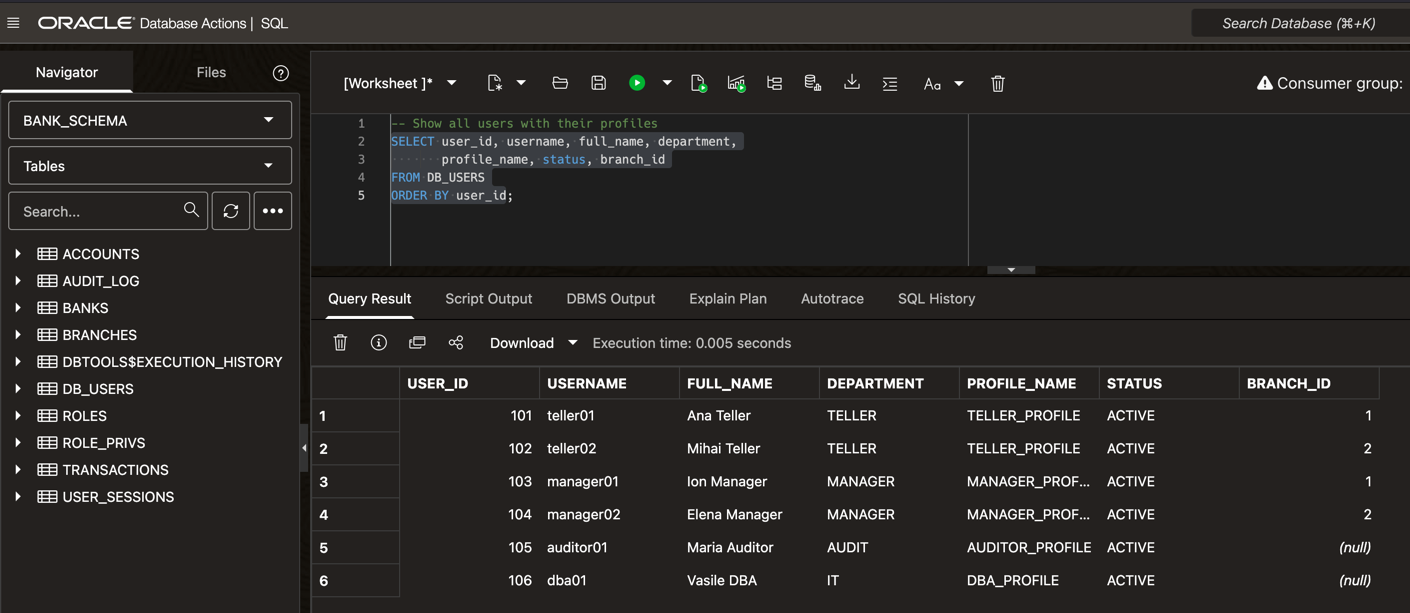
\includegraphics[width=\textwidth]{04-gestiune-identitati/01-user-profiles.png}
    \caption{Profile utilizatori cu limite de resurse}
    \label{fig:matrix-process-user}
\end{figure}

\begin{figure}[H]
    \centering
    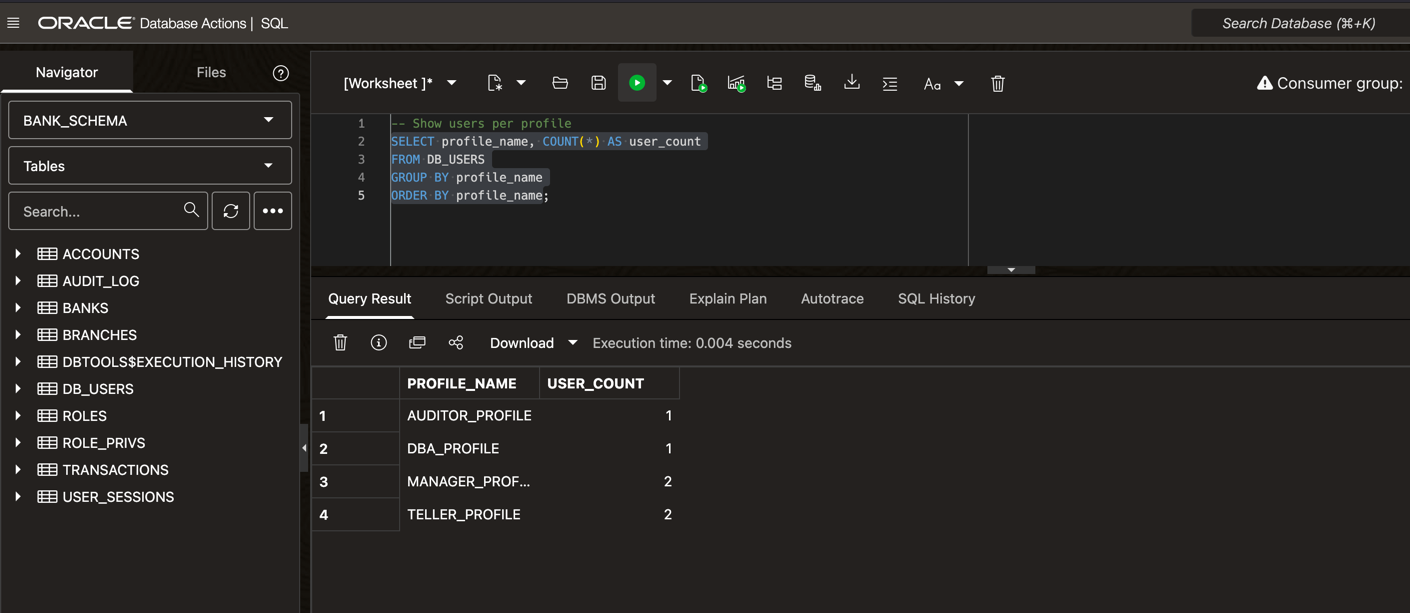
\includegraphics[width=\textwidth]{04-gestiune-identitati/02-profile-summary.png}
    \caption{Rezumat profile și asignarea utilizatorilor}
    \label{fig:profile-summary}
\end{figure}

\textbf{Beneficii}:
\begin{itemize}
    \item Prevenirea atacurilor de tip DoS (limitare resurse)
    \item Segregarea responsabilităților (profiluri diferențiate)
    \item Conformitate cu reglementările bancare (control acces granular)
\end{itemize}

\newpage
\section{Privilegii și roluri}

\subsection{Ierarhia de roluri}

Sistemul implementează un model \textbf{Role-Based Access Control (RBAC)} cu o ierarhie pe 6 niveluri. Fiecare rol moștenește privilegiile rolului părinte, creând o structură piramidală de drepturi.

\textbf{Ierarhia implementată}:
\begin{enumerate}
    \item \textbf{BASE\_EMPLOYEE\_ROLE}: Acces minim (CONNECT, SELECT pe tabele publice)
    \item \textbf{TELLER\_ROLE}: Moștenește BASE + INSERT/UPDATE pe TRANSACTIONS (sume < 5,000 RON)
    \item \textbf{SENIOR\_TELLER\_ROLE}: Moștenește TELLER + limite crescute (< 10,000 RON)
    \item \textbf{MANAGER\_ROLE}: Moștenește SENIOR\_TELLER + DELETE, grant-uri, sume nelimitate
    \item \textbf{AUDITOR\_ROLE}: Ramură separată, acces read-only la toate datele
    \item \textbf{DBA\_ROLE}: Acces complet, administrare sistem
\end{enumerate}

\begin{figure}[H]
    \centering
    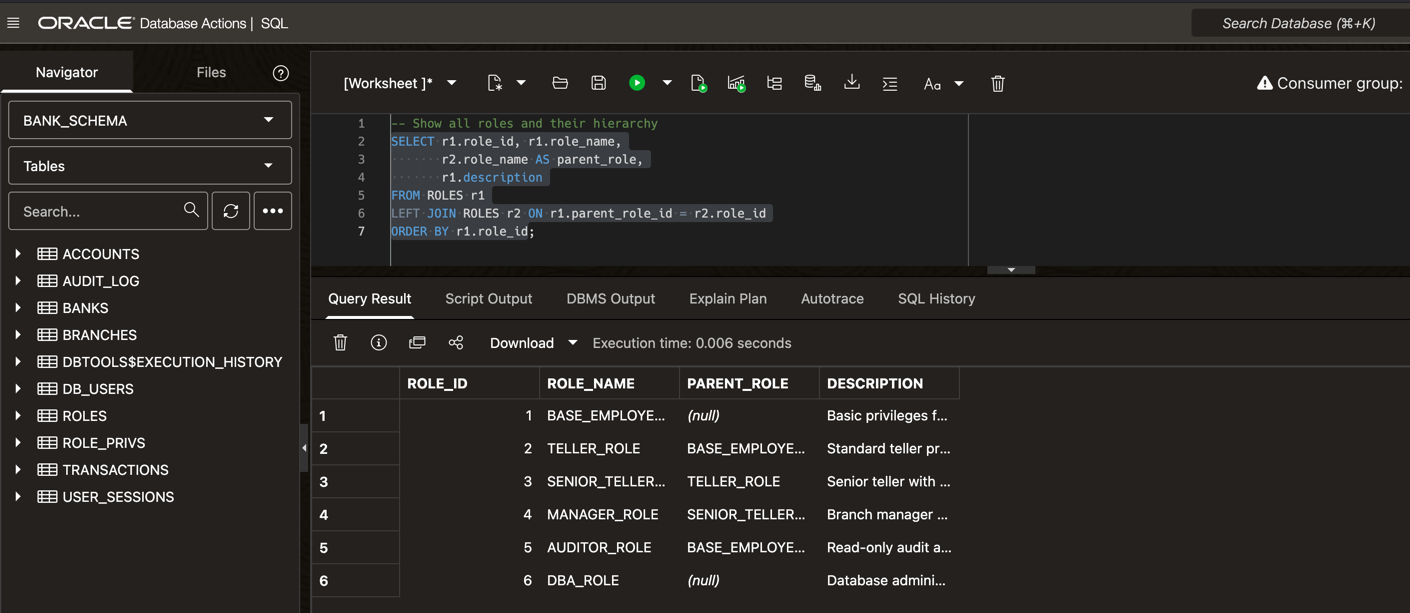
\includegraphics[width=0.9\textwidth]{05-privilegii-roluri/01-role-hierarchy.png}
    \caption{Ierarhia de roluri și moștenirea privilegiilor}
    \label{fig:role-hierarchy}
\end{figure}

\subsection{Privilegii definite}

Proiectul definește \textbf{37 privilegii} distribuite pe cele 6 roluri. Privilegiile includ atât drepturi de sistem (CONNECT, CREATE SESSION) cât și drepturi pe obiecte (SELECT, INSERT, UPDATE, DELETE pe tabele specifice).

\textbf{Tipuri de privilegii}:
\begin{itemize}
    \item \textbf{SYSTEM}: Privilegii de sistem (CONNECT, CREATE SESSION)
    \item \textbf{OBJECT}: Privilegii pe obiecte (SELECT, INSERT, UPDATE, DELETE)
    \item \textbf{GRANTABLE}: Privilegii cu drept de grant (doar pentru manageri și DBA)
\end{itemize}

\begin{figure}[H]
    \centering
    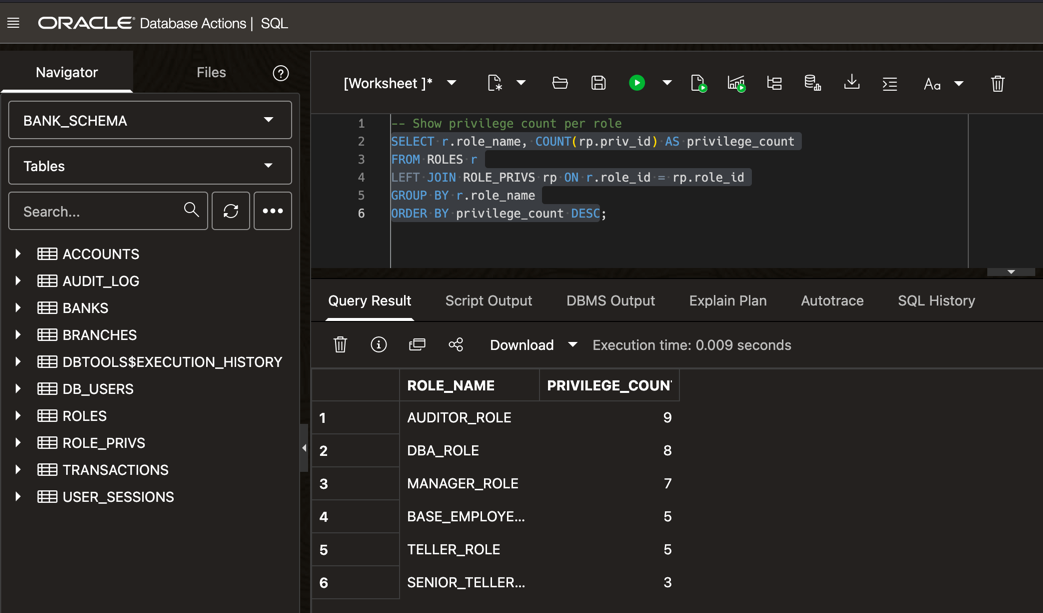
\includegraphics[width=0.9\textwidth]{05-privilegii-roluri/02-privilege-count.png}
    \caption{Distribuția privilegiilor pe roluri}
    \label{fig:privilege-count}
\end{figure}

\begin{figure}[H]
    \centering
    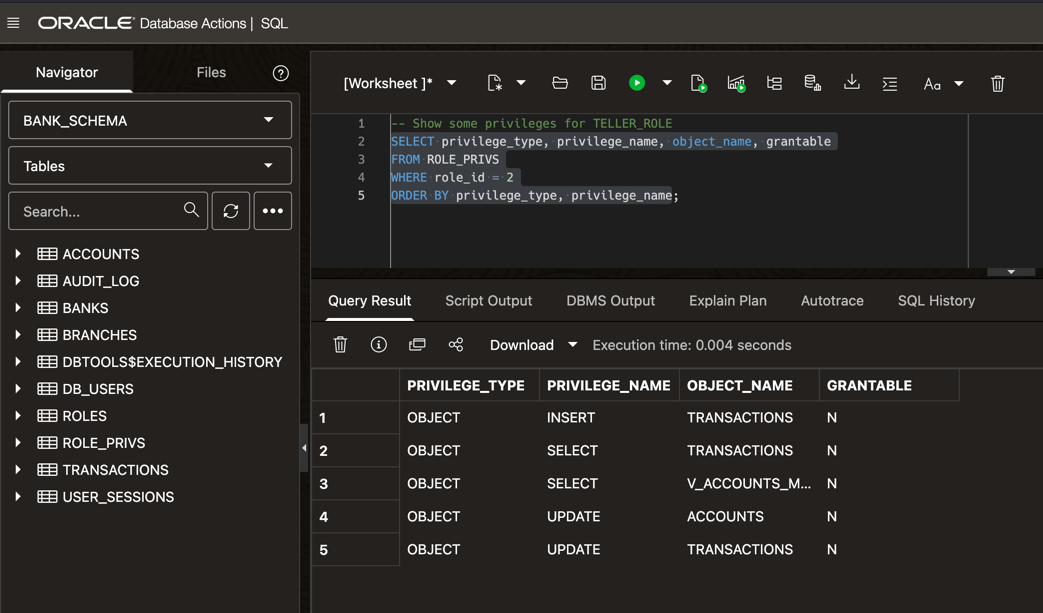
\includegraphics[width=0.9\textwidth]{05-privilegii-roluri/03-sample-privileges.png}
    \caption{Exemple de privilegii și restricții}
    \label{fig:sample-privileges}
\end{figure}

\textbf{Avantaje RBAC}:
\begin{itemize}
    \item Principiul privilegiului minim (least privilege)
    \item Ușurință în administrare (grant pe rol, nu pe utilizator)
    \item Segregarea responsabilităților (separation of duties)
    \item Conformitate cu standardele bancare (Basel III, Romanian Banking Regulations)
\end{itemize}

\newpage
\section{Securitatea aplicațiilor}

\subsection{Protecție împotriva SQL Injection}

SQL Injection este una dintre cele mai periculoase vulnerabilități conform OWASP Top 10 (A03:2021). Proiectul demonstrează diferența dintre cod vulnerabil și cod securizat.

\textbf{Abordare vulnerabilă - Concatenare string-uri}:
\begin{lstlisting}[style=sqlstyle, caption={Procedură vulnerabilă la SQL Injection}]
CREATE OR REPLACE PROCEDURE GET_ACCOUNT_INFO_VULN(
    p_account_number VARCHAR2
) AS
    v_sql VARCHAR2(1000);
BEGIN
    -- PERICOL: Concatenare directă - vulnerabil la injection
    v_sql := 'SELECT * FROM ACCOUNTS WHERE account_number = '''
             || p_account_number || '''';
    EXECUTE IMMEDIATE v_sql;
END;
\end{lstlisting}

\textbf{Abordare securizată - Variabile bind}:
\begin{lstlisting}[style=sqlstyle, caption={Procedură sigură cu variabile bind}]
CREATE OR REPLACE PROCEDURE GET_ACCOUNT_INFO_SECURE(
    p_account_number VARCHAR2
) AS
    v_result ACCOUNTS%ROWTYPE;
BEGIN
    -- SIGUR: Folosește variabile bind
    SELECT * INTO v_result
    FROM ACCOUNTS
    WHERE account_number = p_account_number;
END;
\end{lstlisting}

\begin{figure}[H]
    \centering
    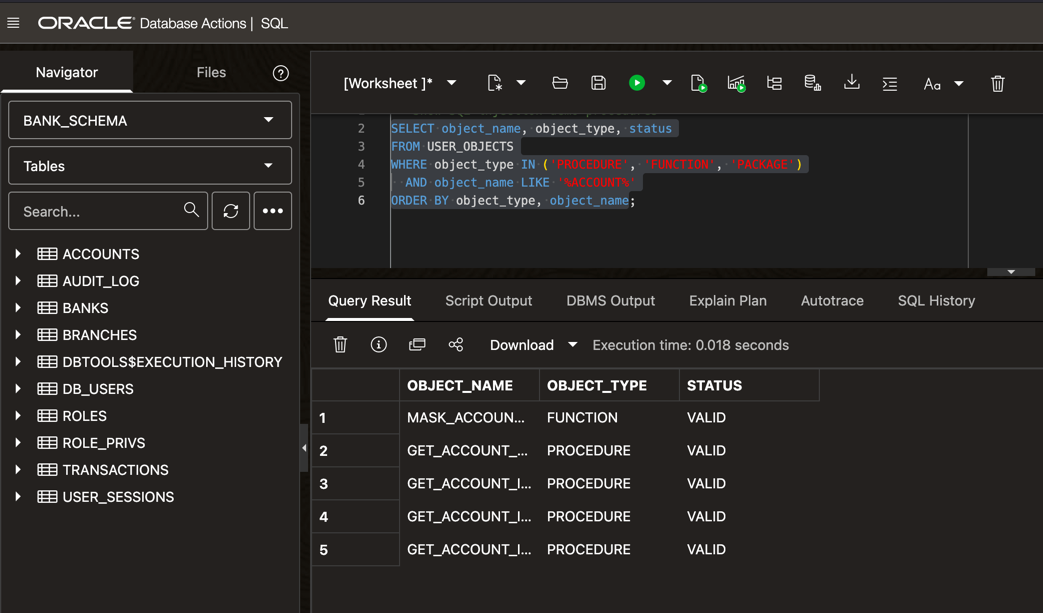
\includegraphics[width=0.9\textwidth]{06-securitate-aplicatii/01-procedures.png}
    \caption{Comparație proceduri vulnerabile vs. sigure}
    \label{fig:sql-injection}
\end{figure}

\textbf{Tehnici de protecție implementate}:
\begin{itemize}
    \item Variabile bind (prevent parametrizare)
    \item DBMS\_ASSERT pentru validare input
    \item Strong typing (declarare tipuri explicite)
    \item Whitelist validation pentru parametri string
\end{itemize}

\subsection{Context aplicație}

Sistemul folosește \textbf{Application Context} pentru a menține starea sesiunii și a valida utilizatorii. Contextul include:
\begin{itemize}
    \item User ID și Branch ID curent
    \item Timestamp sesiune
    \item Validare autentificare
\end{itemize}

\begin{figure}[H]
    \centering
    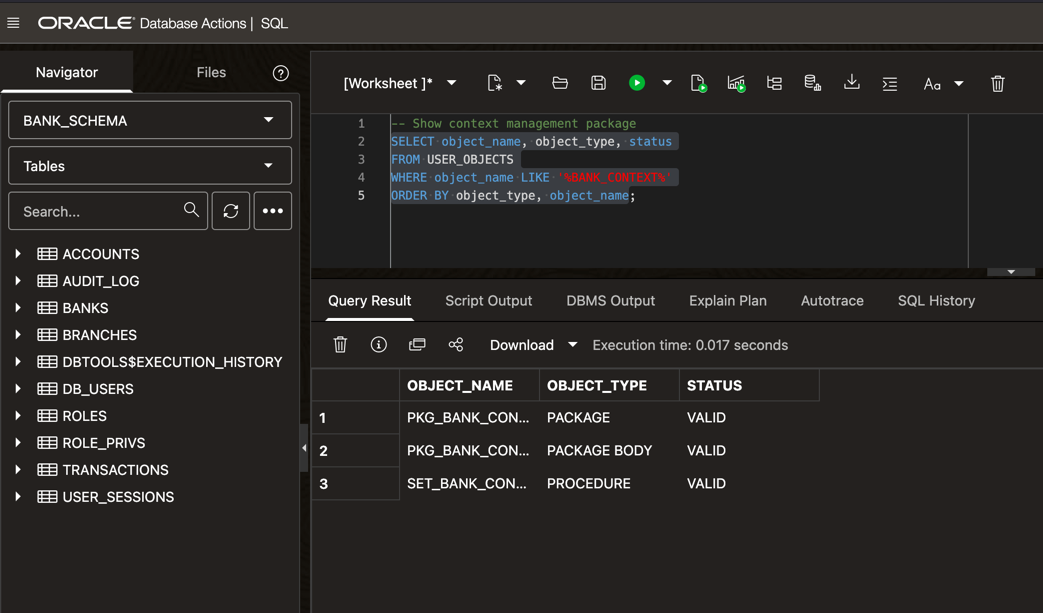
\includegraphics[width=0.9\textwidth]{06-securitate-aplicatii/02-context-package.png}
    \caption{Package pentru gestionarea contextului aplicației}
    \label{fig:context-package}
\end{figure}

\textbf{Nota}: Pe Oracle Autonomous Database, crearea de contexte este restricționată din motive de securitate. Funcționalitatea de bază funcționează, dar setarea contextului necesită privilegii suplimentare indisponibile pe Free Tier.

\newpage
\section{Mascarea datelor}

\subsection{Funcții de mascare}

Data masking protejează datele sensibile prin \textbf{obfuscare parțială}, permițând utilizatorilor neautorizați să vadă structura datelor fără a accesa valorile reale. Sistemul implementează 3 funcții de mascare pentru diferite tipuri de date sensibile.

\textbf{Funcții implementate}:

\begin{enumerate}
    \item \textbf{MASK\_ACCOUNT\_NUMBER}: Maskează numere IBAN
    \begin{itemize}
        \item Input: RO49AAAA1B31007593840001
        \item Output: RO49************0001
        \item Păstrează primele 4 și ultimele 4 caractere
    \end{itemize}

    \item \textbf{MASK\_EMAIL}: Maskează adrese email
    \begin{itemize}
        \item Input: andrei.vasilescu@email.com
        \item Output: a***************@email.com
        \item Păstrează prima literă și domeniul
    \end{itemize}

    \item \textbf{MASK\_PHONE}: Maskează numere de telefon
    \begin{itemize}
        \item Input: +40721234567
        \item Output: +407********67
        \item Păstrează prefix țară și ultimele 2 cifre
    \end{itemize}
\end{enumerate}

\begin{figure}[H]
    \centering
    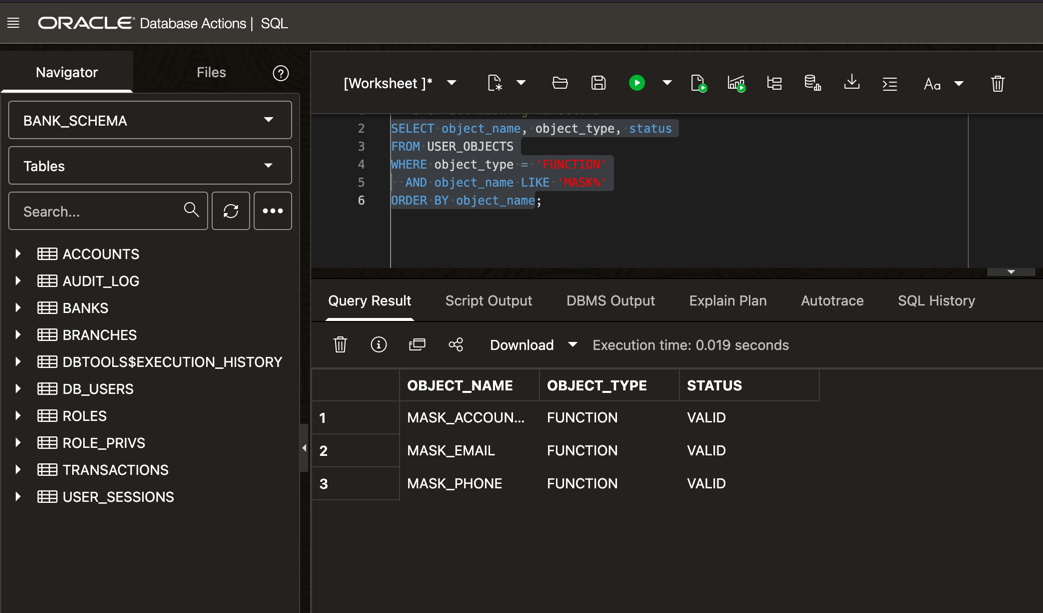
\includegraphics[width=0.9\textwidth]{07-mascare-date/01-masking-functions.png}
    \caption{Definirea funcțiilor de mascare}
    \label{fig:masking-functions}
\end{figure}

\subsection{View-uri mascate}

Sistemul creează \textbf{view-uri securizate} care aplică automat funcțiile de mascare. Utilizatorii cu privilegii reduse primesc acces doar la view-urile mascate, în timp ce managerii și auditorii văd datele nemascate.

\textbf{View-uri create}:
\begin{itemize}
    \item \textbf{V\_ACCOUNTS\_MASKED}: Conturi cu numere IBAN mascate
    \item \textbf{V\_USERS\_MASKED}: Utilizatori cu email și telefon mascate
\end{itemize}

\begin{figure}[H]
    \centering
    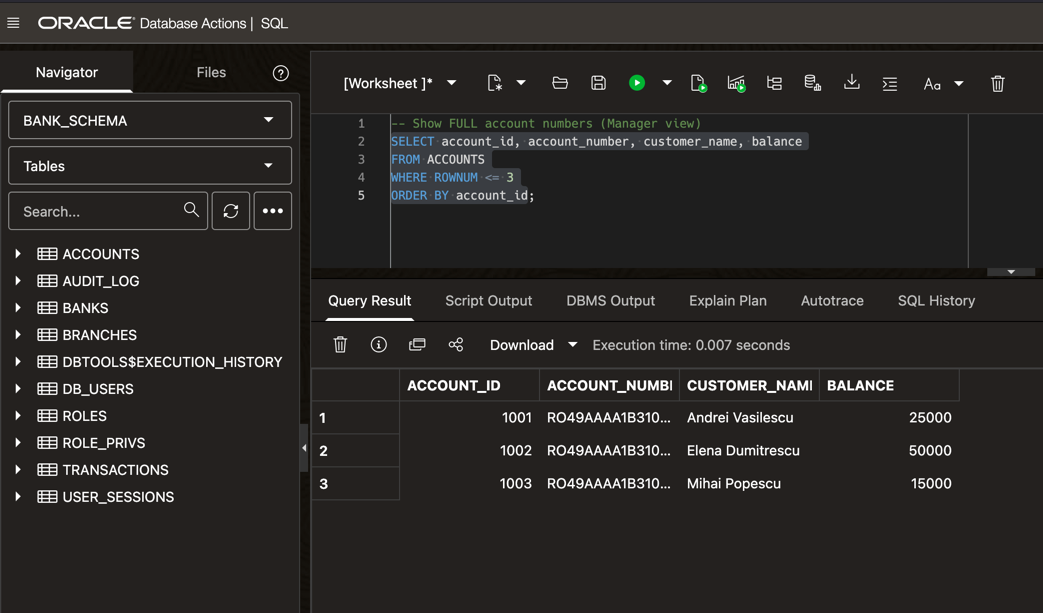
\includegraphics[width=0.9\textwidth]{07-mascare-date/02-unmasked-view.png}
    \caption{Date nemascate - acces complet (manageri, auditori)}
    \label{fig:unmasked}
\end{figure}

\begin{figure}[H]
    \centering
    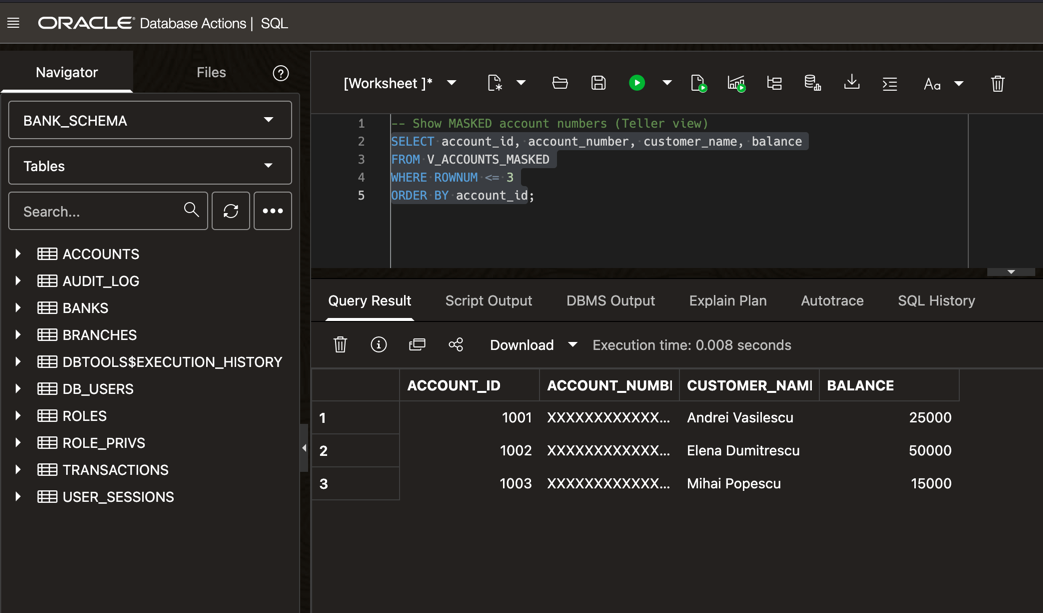
\includegraphics[width=0.9\textwidth]{07-mascare-date/03-masked-view.png}
    \caption{Date mascate - acces restricționat (casieri, angajați)}
    \label{fig:masked}
\end{figure}

\begin{figure}[H]
    \centering
    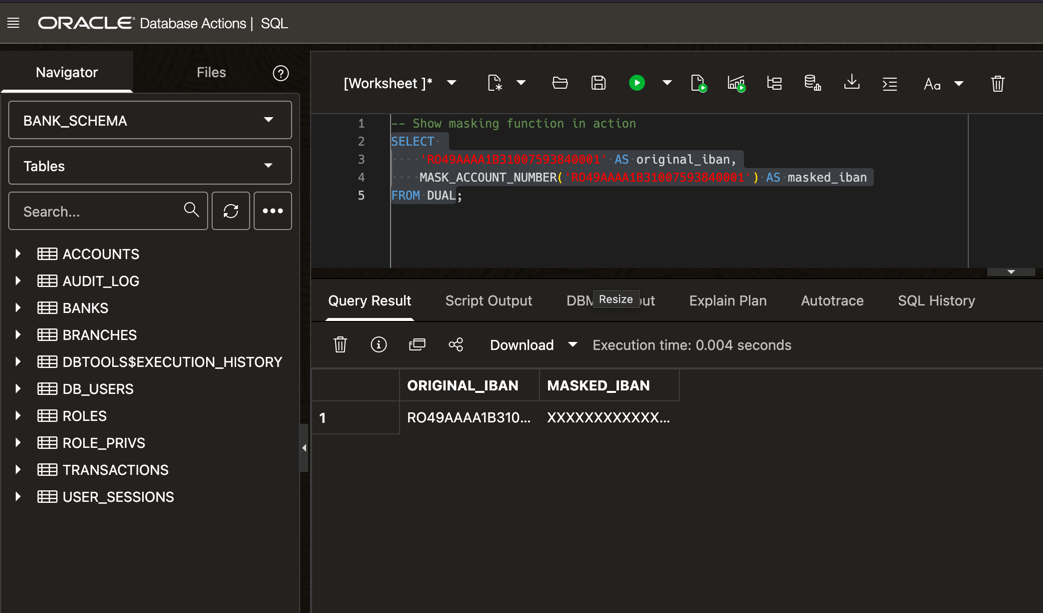
\includegraphics[width=0.9\textwidth]{07-mascare-date/04-masking-test.png}
    \caption{Test funcționare mascare - comparație side-by-side}
    \label{fig:masking-test}
\end{figure}

\textbf{Cazuri de utilizare}:
\begin{itemize}
    \item Dezvoltatori testând cu date de producție
    \item Support tehnic cu acces limitat
    \item Rapoarte și analize fără dezvăluire date personale
    \item Conformitate GDPR (minimizarea accesului la date personale)
\end{itemize}

\newpage
\section{Complexitate și securitate avansată}

\subsection{Virtual Private Database (VPD)}

\textbf{Virtual Private Database (VPD)} implementează securitate la nivel de rând (row-level security) prin aplicarea automată de predicare WHERE la query-uri. Fiecare utilizator vede doar rândurile pentru care are permisiune, fără modificări la nivel de aplicație.

\textbf{Implementare}:
\begin{itemize}
    \item \textbf{Policy}: VPD\_ACCOUNTS\_BRANCH\_POLICY
    \item \textbf{Funcție}: FN\_BRANCH\_SECURITY
    \item \textbf{Scop}: Casierii văd doar conturile din sucursala lor
\end{itemize}

\textbf{Logica de securitate}:
\begin{lstlisting}[style=sqlstyle, caption={Funcție VPD pentru filtrare rânduri}]
CREATE OR REPLACE FUNCTION FN_BRANCH_SECURITY(
    schema_owner VARCHAR2,
    object_name VARCHAR2
) RETURN VARCHAR2 IS
    v_branch_id NUMBER;
    v_predicate VARCHAR2(2000);
BEGIN
    -- Caută branch_id utilizatorului curent
    SELECT branch_id INTO v_branch_id
    FROM DB_USERS
    WHERE username = SYS_CONTEXT('USERENV', 'SESSION_USER');

    -- Returnează predicat de filtrare
    RETURN 'branch_id = ' || v_branch_id;
END;
\end{lstlisting}

\begin{figure}[H]
    \centering
    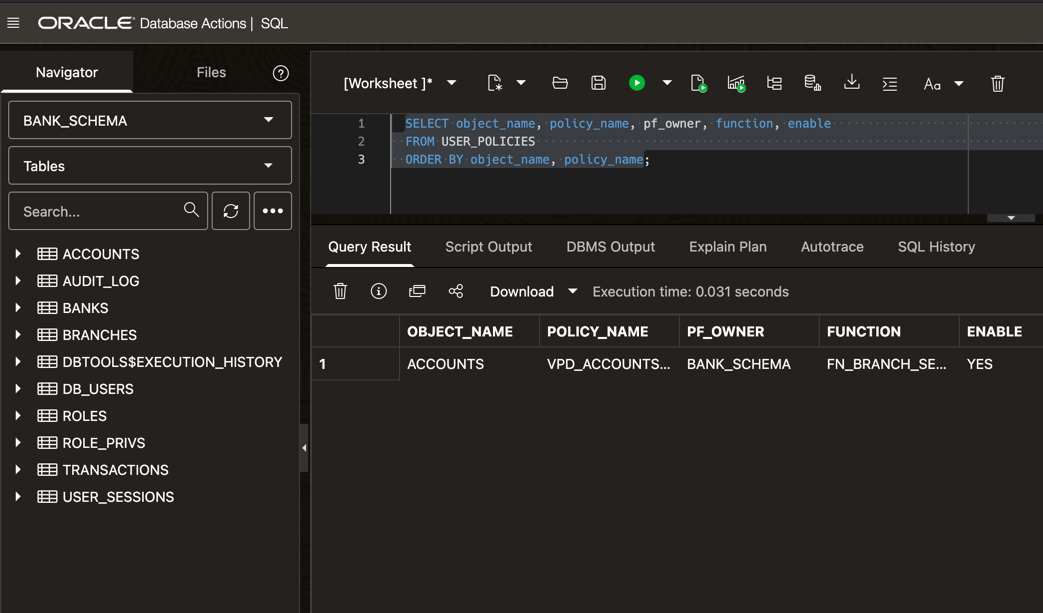
\includegraphics[width=0.9\textwidth]{08-complexitate/01-vpd-policy.png}
    \caption{Policy VPD aplicată pe tabelul ACCOUNTS}
    \label{fig:vpd-policy}
\end{figure}

\textbf{Avantaje VPD}:
\begin{itemize}
    \item Transparent pentru aplicație (nu necesită modificări cod)
    \item Imposibil de bypass (aplicat la nivel de kernel Oracle)
    \item Performant (Oracle optimizează query-urile automat)
    \item Centralizat (logica de securitate în baza de date, nu în aplicație)
\end{itemize}

\subsection{Dashboard securitate}

Sistemul include un \textbf{view analitic} care agregă metrici de securitate din întreaga bază de date. Dashboard-ul oferă o vedere de ansamblu asupra:

\textbf{Metrici monitorizate}:
\begin{itemize}
    \item Coloane criptate (TDE)
    \item Trigger-uri de audit active
    \item Policy-uri VPD aplicate
    \item Roluri și privilegii definite
    \item Sesiuni active per utilizator
    \item View-uri de mascare date
\end{itemize}

\begin{figure}[H]
    \centering
    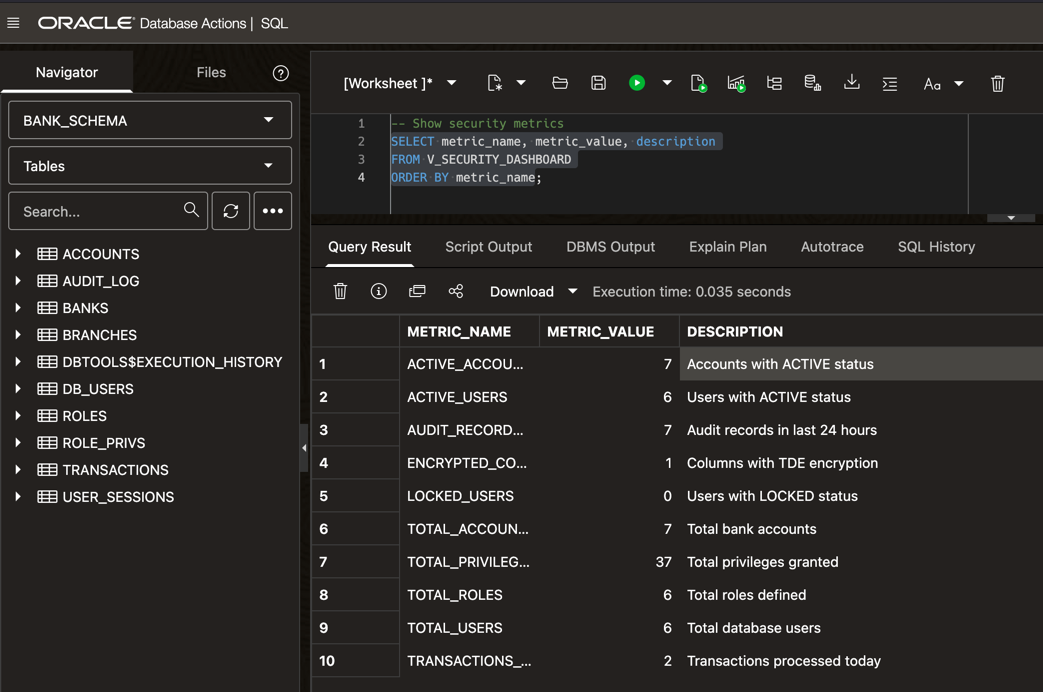
\includegraphics[width=0.9\textwidth]{08-complexitate/02-security-dashboard.png}
    \caption{Dashboard securitate - overview complet}
    \label{fig:security-dashboard}
\end{figure}

\textbf{Utilitate dashboard}:
\begin{itemize}
    \item Monitorizare continuă a posturii de securitate
    \item Raportare rapidă pentru audituri
    \item Detectare configurări lipsă sau incorecte
    \item Bază pentru Security Information and Event Management (SIEM)
\end{itemize}

\newpage
\section{Concluzii}

Proiectul demonstrează implementarea unui sistem bancar securizat folosind \textbf{toate conceptele majore de securitate a bazelor de date}.

\textbf{Cerințe N1 (Nota de trecere)}:
\begin{itemize}
    \item[$\checkmark$] Schemă bază de date (9 tabele, 68 constrângeri, 13 indexuri)
    \item[$\checkmark$] Criptare date (TDE pe coloana BALANCE)
    \item[$\checkmark$] Auditare bază de date (Trigger-uri + FGA + Audit Log)
    \item[$\checkmark$] Gestiunea identităților (6 profile, matrici de acces)
    \item[$\checkmark$] Mascare date (3 funcții, 2 view-uri mascate)
\end{itemize}

\textbf{Cerințe N2 (Nota mai mare)}:
\begin{itemize}
    \item[$\checkmark$] Privilegii și roluri (37 privilegii, ierarhie cu 6 roluri)
    \item[$\checkmark$] Protecție SQL Injection (Variabile bind, DBMS\_ASSERT)
\end{itemize}

\textbf{Cerințe N3 (Nota maximă)}:
\begin{itemize}
    \item[$\checkmark$] Funcționalități complexe (VPD, dashboard securitate, analiză)
    \item[$\checkmark$] Documentație completă (Acest raport)
\end{itemize}

\subsection{Statistici proiect}

\begin{table}[H]
\centering
\begin{tabular}{ll}
\toprule
\textbf{Metric} & \textbf{Value} \\
\midrule
Total Lines of Code & 4,308 lines SQL \\
Total Database Objects & 50+ objects \\
Security Layers & 5 layers \\
Compliance Standards & 4 (GDPR, PCI-DSS, OWASP, Banking) \\
Encrypted Columns & 1 (BALANCE) \\
Audit Policies & 5 (4 triggers + 1 FGA) \\
User Profiles & 6 profiles \\
Roles Defined & 6 roles \\
Privileges Defined & 37 privileges \\
Tables Created & 9 tables \\
Views Created & 5 views \\
Functions Created & 6 functions \\
\bottomrule
\end{tabular}
\caption{Statistici proiect}
\label{tab:stats}
\end{table}

\subsection{Compliance standards met}

\begin{itemize}
    \item[$\checkmark$] \textbf{GDPR Article 32} - Security of processing
    \item[$\checkmark$] \textbf{PCI-DSS Requirements 3, 6, 7, 8, 10} - Acoperire completă
    \item[$\checkmark$] \textbf{OWASP Top 10 - A03:2021} - Injection prevention
    \item[$\checkmark$] \textbf{Romanian Banking Regulations} - Segregation of duties
\end{itemize}

\newpage
\begin{thebibliography}{9}

\bibitem{oracle-security}
Oracle Corporation. (2024).
\textit{Oracle Database Security Guide 19c}.
Oracle Documentation.

\bibitem{oracle-tde}
Oracle Corporation. (2024).
\textit{Oracle Advanced Security Transparent Data Encryption}.
Oracle White Paper.

\bibitem{pci-dss}
Payment Card Industry Security Standards Council. (2024).
\textit{PCI DSS v4.0 Requirements and Testing Procedures}.

\bibitem{gdpr}
European Parliament. (2016).
\textit{General Data Protection Regulation (GDPR) - Article 32}.

\bibitem{owasp}
OWASP Foundation. (2021).
\textit{OWASP Top 10:2021 - A03 Injection}.

\bibitem{oracle-plsql}
Oracle Corporation. (2024).
\textit{Oracle Database PL/SQL Packages and Types Reference 19c}.

\end{thebibliography}

\end{document}
